  \subsection{Leptonic $W^{\pm}$-decay}
  \begin{itemize}
    \item The decay width $Γ$ is proportional to the square of the matrix element $|M|^2$, which is proportional to the square of the coupling constant $g_{W}^2$.
    \item As $m_{W} ≫ m_e ≫ m_{ν_e}$, it is the most important energy. 
    \item The natural width has units of energy, and is given by $Γ(W^{-} → e^{-} \bar{ν}_e) ∝ g^2_{W}m_{W}c^2$ which approximates to $α_{W}20$ GeV $= 0.223$ GeV. This gives $α_{W} ≈ 1/238$. This is a lot smaller than $α_{\text{EM}} = 1/137$
  \end{itemize}
  
  
  \subsection{Cabibbo Suppression}
  \paragraph{Cabibbo allowed process:} Has a matrix element $\left|V_{f_1f_2}\right|^2$ as seen in the quark mixing matrix defined in \cref{eq: quark_mixing}, which is approximately 1. 
  \paragraph{Cabibbo suppressed process:} Has a matrix element $\left|V_{f_1f_2}\right|^2$ as defined in \cref{eq: quark_mixing}, which is much smaller than 1.

  The ratio between the Kaon and Pion decay as depicted in \cref{fig: kaon_pion_decay} has a width ratio proportional to their couplings. We know from the linear combinations of the strange and down quarks that we get the following couplings:
  \begin{equation}
    d' = d \cos θ_c + s \sin θ_c → g_{ud} = q_{W}\cos θ_c
  \end{equation}
  \begin{equation}
    s' = -d \sin θ_c + s \cos θ_c → g_{us} = q_{W}\sin θ_c
  \end{equation}
  \begin{equation}
    \frac{Γ(K^{-} → μ^{-} \bar{ν}_{μ})}{Γ(π^{-} → μ^{-} \bar{ν}_{μ})} = \frac{g^2_{us}}{g^2_{ud}} = \tan^2 θ_c
  \end{equation}

\begin{figure}[h!]
\centering
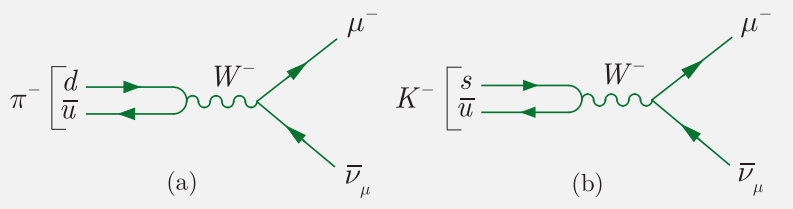
\includegraphics[width = .8\textwidth]{kaon_pion_decay.png}
\caption{Pion (a) and Kaon (b) decay through a charged weak interaction.}
\label{fig: kaon_pion_decay}
\end{figure}


\subsection{Charm Decays}   
\begin{itemize}
    \item From experiment we know $θ_{c} \approx 13 ^∘$
    \item As $\cos ^2 θ_c \approx 1$ and $\sin ^2 θ_c \approx 0$, we can roughly say that $d' \approx d$ and $s' \approx s$
    \item As a result of lepton-quark symmetry, we get: 
    \begin{itemize}
        \item $W^{+} → c \bar{s}$ and $W^{-} → u \bar{d}$ being \textbf{Cabibbo allowed}
        \item $W^{+} → c \bar{d}$ and $W^{-} → u \bar{s}$ being \textbf{Cabibbo suppressed}
    \end{itemize}
\end{itemize}

\subsubsection{Charmed Hadron Decays}
Given that $c → s'W^{+}$ we can expand that to $s'W^{+} = s \cos θ_c W^{+} - d \sin θ_c W^{+}$. Using the approximations from above, we can say that the charmed quark almost always decays into a strange quark.

\subsection{Selection Rules for Charged Weak Decays}
\subsubsection{Selection rules applied to hadronic part of charged weak decays}
\begin{itemize}
    \item The rules are derived from experiment. The capital letters denote if a quark is an up (U) or down (D) type quark. 
    \item \textbf{Semi-leptonic}: $D → W^{-} U$ or $\bar{U} → W^{-} \bar{D}$ followed by $W^{-} →  l^{-} \bar{ν}_l$
    \item Both of these have $ΔQ = +1$ to balance the charge of $W^{-}$. 
    \item We can have $d → W^{-} u$ or $\bar{u} → W^{-} \bar{d}$ which gives $ΔS = 0$
    \item We can also have $s → W^{-}u$ or $\bar{u} →  W^{-} \bar{s}$
\end{itemize}

\subsubsection{Semi-Leptonic Charged Weak Decays (\cref{fig: semi-leptonic_charged_weak_decays})} 
\begin{itemize}
    % \item
    \parbox[t]{\dimexpr\textwidth-\leftmargin}{
    \vspace{-7.5mm}
    \begin{wrapfigure}{R}{0.4\textwidth}
    \vspace{-5mm}
    \centering
    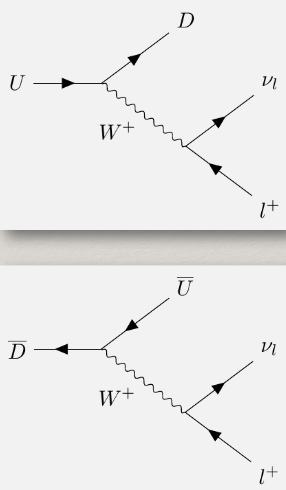
\includegraphics[width = .25\textwidth]{semi-leptonic_charged_weak_decays.png}
    \caption{}
    \label{fig: semi-leptonic_charged_weak_decays}
  \end{wrapfigure}
  
  \item $\bar{D} → W^{+} \bar{U}$ or $U → W^{+} D$ followed by $W^{+} → l^{+} ν_l$
  \item Both are $ΔQ = -1$ to balance the charge of $W^{+}$
  \item We can have $\bar{d} → W^{+} \bar{u}$ or $u → W^{+} d$ which gives $ΔS = 0$
  \item We can also have $\bar{s} → W^{+} \bar{u}$ or $u → W^{+} s$ which gives $ΔS = -1$
  \item In total we have $ΔS = 0$ with $ΔQ = ±1$ and $ΔS = ΔQ = ±1$. 
    \item There is no $ΔS = ±2$    
    }
  \end{itemize}
  
  
\vspace{0.5mm}
\subsubsection{Fully Hadronic Charged Weak Decays (\cref{fig: fully_hadronic_charged_weak_decays})}
\begin{figure}[ht!]
    \centering
    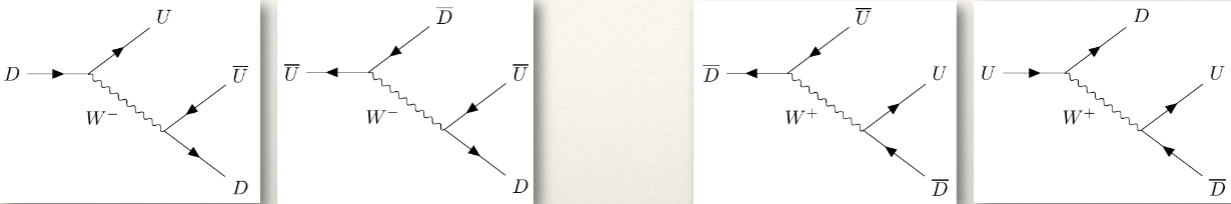
\includegraphics[width = .8\textwidth]{fully_hadronic_charged_weak_decays.png}
    \caption{Decay by the $W^{-}$ on the left, and by the $W^{+}$ on the right.}
    \label{fig: fully_hadronic_charged_weak_decays}
    \end{figure}

\begin{itemize} 
  \item Looking at the left side of \cref{fig: fully_hadronic_charged_weak_decays}:
  \begin{itemize}
    \item $ΔQ = 0$ by construction. 
    \item We can have $ΔS = 0$ or $ΔS = +1$ at the let vertices. 
    \item At the right vertices we can have $ΔS = 0$ or $ΔS = -1$. 
    \item All together we can have $ΔS = 0$ or $ΔS = ±1$
  \end{itemize}
  \item Looking at the right side of \cref{fig: fully_hadronic_charged_weak_decays}:
  \begin{itemize}
    \item $ΔQ = 0$ by construction.
    \item At the left vertices we can have $ΔS = 0$ or $ΔS = -1$.
    \item At the right vertices we can have $ΔS = 0$ or $ΔS = +1$.
    \item All together we can have $ΔS = 0$ or $ΔS = ±1$
  \end{itemize}
\end{itemize}

\subsubsection{Summary}
\begin{itemize}
  \item Selection rules apply to hadronic parts of decay. 
  \item \textbf{Semi-leptonic}: $ΔS = 0$ and $ΔQ = ±1$ and $ΔS = ΔQ = ±1$
  \item \textbf{Fully Hadronic}: $ΔS = 0$ or $ΔS = ±1$ with $ΔQ = 0$
  \item There is no $ΔS = ±2$
  \item There is no $Δs = -ΔQ = ±1$
  \item The above is derived from allowed $W^{±}$ and $S(s) = -S(\bar{s}) = -1$
\end{itemize}

\subsubsection{Consequence of Selection Rules}
Hadrons with multiple unstable quarks that decay weakly, decay in cascades. This means that particles which comes as a product from a decay, can decay further.

\paragraph{Example:}
The $π^{0}$ decays into two photons almost instantly.
\begin{align}
  \begin{aligned}
  &Ω^{-}(sss) → &&\underset{↓}{Ξ}^0(uss) + π^{-}(\bar{u}d) \\ 
  %
   &&&\begin{aligned}
      Ξ^{0} (uss) → &\underset{↓}{Λ}^{0}(uds) + π^{0}(\bar{u}u)\\ 
    %
      &\begin{aligned}
        Λ^{0} (uds) → p(uud) 
      \end{aligned}\\
    %
    \end{aligned}\\ 
  %
   &+ π^{-}(\bar{u}d)
\end{aligned}
\end{align}

\subsection{Three Generations}
\begin{itemize}
  \item We apply the letpon-quark symmetry to all generations $\begin{pmatrix*}[r]
   U \\
   D \\
  \end{pmatrix*}$. 
  \item A first approximation matrix is given by:
  \begin{equation}
    \begin{pmatrix*}[r]
     d' \\
     s' \\
     b' \\
    \end{pmatrix*} = 
    \begin{pmatrix*}[r]
      \cos θ_c & \sin θ_c & 0 \\
      -\sin θ_c & \cos θ_c & 0 \\
      0 & 0 & 1 \\
    \end{pmatrix*} 
    \begin{pmatrix*}[r]
      d \\
      s \\
      b \\
    \end{pmatrix*} = 
    \begin{pmatrix*}[r]
     V_{ud} & V_{us} & V_{ub} \\
     V_{cd} & V_{cs} & V_{cb} \\
     V_{td} & V_{ts} & V_{tb} \\
    \end{pmatrix*}
  \end{equation}
  \item Since the top quark is much heavier than the down quark, one could think the bottom quark is stable, but it is not. $τ_b ≈ 10^{-12}$s. 
  \item From measurements we know $\left|V_{ub}\right|^2 = 1.55 ⋅ 10^{-5}$, and $\left|V_{cb}\right|^2 = 1.78 ⋅ 10^{-3}$.
  \item As $\left|V_{cb}\right|^2$ is so much larger than $\left|V_{ub}\right|^2$, we can say the the bottom quark decays into a charm quark almost always.
  \item This is only a first approximation. In actuality, the top quark can sometimes decay into down and strange quarks, as the matrix above implies is impossible. The bottom quark also has a short lifetime. It is not zero. 
  \item The top quark have such a short lifetime $τ_{t} = 4 ⋅ 10^{-25}$, that light can't travel the single femto meter required for bonding to occur. The light would use approximately $10^{-23}$s, in which the top quark has decayed. There exist no top quark hadrons. 
  \item On the second row, we see the charm quark does not decay into the bottom quark due to its smaller mass. As the angle $θ_{c}$ is small, it most often decays to a strange quark, instead of a down quark. 
  \item When multiple strange, charmed and bottom quarks are present, they decay in cascades.
\end{itemize}

\subsection{Part 1 Essentials}
\begin{itemize}
  \item Inderstand what is meant by lepton-universality, lepton-quark symmetry and quark mixing, for the charged weak interaction.
  \begin{itemize}
    \item Apply these to find approximate rations of decay widths and cross-sections. 
  \end{itemize}
  \item Be able to sketch the main features of the quark-mixing matrix. 
  \begin{itemize}
    \item How does this influence quark and hadron decays?
  \end{itemize} 
  \item Be able to explain the origin of the "selection rules" for charged weak decays of hadrons. 
  \begin{itemize}
    \item Selection rules are one of the few things worth memorizing. Especially strangeness $Δs ∈ \left\{-1,0,1\right\}$
  \end{itemize}
\end{itemize}

\subsection{Electroweak Unification and the Higgs boson}
\subsubsection{Gauge Invariance}
\paragraph{Definition:} Gauge invariance means that the laws of physics behave the same way no  matter how you measure something. An example would be how the phase of a wavefunction $ψ = ψ_0e^{iθ}$ does to change the probability density $|ψ|^2 = |ψ_0|^2$. 

\textbf{It is not a symmetry of nature, but a redundancy in the description of nature.}

\begin{itemize}
  \item \textbf{Gauge invariance} and spontaneous symmetry breaking are the two main principles of the electroweak theory.
  \item \textbf{Gauge principle}: Propose a gauge (phase) transformation of the wavefunction and add an interaction so that the gauge remains unobservable. 
\end{itemize}

\paragraph{Gauge Invariance and EM}
  Fields in EM: 
  \begin{equation}
  \vec{B} = \vec{∇} × \vec{A} \quad , \quad  \vec{E} = - \vec{∇}ϕ - \frac{1}{c}\frac{∂ \vec{A}}{∂ t}
  \end{equation}

  Gauge transformations of potential $ϕ$ and vector potential 
  \begin{equation}
    \vec{A} (ϕ, \vec{A}) → (ϕ, \vec{A})' →  \left(ϕ - \frac{1}{c}\frac{∂ α}{∂ t}, \vec{A} + \vec{∇}α\right)    
  \end{equation}
  where $α(t, \vec{h})$ is a doubly differentiable function.

  This gives 
  \begin{equation}
    \vec{B}' = \vec{∇} × \vec{A}' = \vec{∇} × \left(\vec{A} + \vec{∇}α\right) = \vec{∇} × \vec{A} + \vec{∇} × \vec{∇}α 
  \end{equation}
  The last cross product gives: 
  \begin{equation}
    \vec{∇} × \vec{∇}α ≡ 0
  \end{equation}
  as it is the curl of a scalar field. This means $\vec{B} = \vec{B}' = \vec{∇} × \vec{A}$
  Adding this back into the electric field we get:
  \begin{equation}
    \vec{E}' = - \vec{∇} \left(ϕ - \frac{1}{c}\frac{∂ α}{∂ t}\right) - \frac{1}{c}\frac{∂}{∂ t} \left(\vec{A} + \vec{∇}α\right) = - \vec{∇}ϕ - \frac{1}{c}\frac{∂ \vec{A}}{∂ t} + \frac{1}{c}\left( \underbrace{\vec{∇} \frac{∂ α}{∂ t} - \frac{∂}{∂ t} \vec{∇}α}_{0}\right)
  \end{equation}
  \begin{equation}
    \vec{E}' = - \vec{∇}ϕ - \frac{1}{c}\frac{∂ \vec{A}}{∂ t} = \vec{E}
  \end{equation}
  This shows that the electric and magnetic field are unaffected by the gauge transformation $(ϕ,\vec{A}) → (ϕ,\vec{A})'$. With gauge symmetry we get the conservation of charge.

  \subsubsection{Statndard Model Gauge Interactions}
  \begin{itemize}
    \item Introduce locale gauge (phase) transformation. 
    \item \textbf{QED:} $ψ → e^{-iqα(\vec{x})}ψ$, gives a photon. 
    \item \textbf{QCD:} $ψ → e^{-iqα(\vec{x}) ⋅ T_{a}}ψ$, with $T_a = $ 8 color matrices (3X3) gives 8 gluons.
    \item \textbf{Electroweak:} $ψ → e^{-ig'α(\vec{x}) ig \vec{τ} \vec{Λ}(\vec{x})}$ with $\vec{τ} = $3 Pauli matrices, $g'$ the coupling to weak hypercharge singlet ($B^{0}$) and $g$ the coupling to weak isospin triplet ($W^{± /0}$).
    \item The choice of gauge symmetry determines dynamics of the system. 
  \end{itemize}

  \subsubsection{Electoweak Unification/Mixing}
  \begin{itemize}
    \item \textbf{Mixing Hypothesis}: What if the basis of nature is not the $B^{0}$ and $W^{±}$-boson, but the photon and $Z^{0}$-boson?:
    \begin{equation}
      \begin{pmatrix*}[r]
        γ \\
        Z^{0} \\
      \end{pmatrix*} = 
      \begin{pmatrix*}[r]
        \cos θ_{W} & \sin θ_{W} \\
        -\sin θ_{W} & \cos θ_{W} \\
      \end{pmatrix*}
      \begin{pmatrix*}[r]
        B^{0} \\
        W^{±} \\
      \end{pmatrix*}
    \end{equation}
    \item The mixing angle $θ_{W}$ (Weinberg angle) is defined by $\cos θ_{W} ≡ m_{W} / m_{Z}$
    \item Unification condition: $e = g \sin θ_{W} = g' \cos θ_{W}$ with massless photon without any neutrino interactions. 
    \item Gauge symmetry removes divergence in the center mass energy $\sqrt{s}$ when adding the contribution from the photon and $Z^{0}$-boson.
    \item A divergence-free theory is a renormalizable theory. An important property. 
  \end{itemize}
  
\subsubsection{Other Predicitons}
\begin{itemize}
  \item There can be mathematical anomalies in as long as the sum of the lepton charges and  the number of colors charges times the sum of quark charges is zero. 
  \begin{equation}
    ∑_{l}^{} Q_l + 3 ∑_{q}^{} Q_q = 0
  \end{equation}
  \item The standard model can have more generations, but have been adapted to the three observed. 
  \item At low energies we get:
  \begin{equation}
    G_{W} ≡ G_{F} = \frac{(ℏc)^2 \sqrt{2}g^2_{W}}{m^2_{W}c^4}  \quad , \quad  G_{Z} = \frac{(ℏc)^2 \sqrt{2}g^2_{Z}}{m^2_{Z}c^4}
  \end{equation}
  With a ration:
  \begin{equation}
    \frac{G_{Z}}{G_{F}} = \frac{\sin ^2θ}{\cos ^2θ}\cos ^2θ = \sin ^2θ_{W} ≈ 0.21
  \end{equation}
  As the angle is so small, some conclude the $G_{Z} = G_{F}$.
  \item In experiment we get a ratio of $1/3$, which does not match with the theory of $\sin^4 θ_{W} ≈ 0.05$
\end{itemize} 